\documentclass[a4paper, twocolumn]{article}

\author{14231016 马琛骁}
\title{San Fransisco Crime Report}

\usepackage{xeCJK}
\setCJKmainfont{Songti SC}
\usepackage{indentfirst}

\usepackage{listings}

\usepackage[superscript]{cite}
\makeatletter % changes the catcode of @ to 11
\renewcommand\@citess[1]{\textsuperscript{[#1]}}
\makeatother % changes the catcode of @ back to 12

\usepackage{amsmath}

\renewcommand\tablename{表}
\renewcommand\figurename{图}

\begin{document}

\maketitle

\section{数据概览}

训练数据共有 878049 条,每条有 9 个属性,分别统计这些属性值的可能选项如表\ref{tab:train}所示。

\begin{table}[h]
    \centering
    \begin{tabular}{*{5}{r}}
        \hline
        Total& Date& Cate& Dspt& DOW \\
        \hline
        878049& 389257& 39& 879& 7 \\
        1& 2& 22514& 999& 125436 \\
        \hline
        \hline
        Pd& Res& Add& X& Y \\
        \hline
        10& 17& 23228& 34243& 34243 \\
        87805& 51650& 38& 26& 26 \\
        \hline
    \end{tabular}
    \caption{训练集属性}
    \label{tab:train}
\end{table}

测试数据共有 65499 条,每条有 6 个属性,分别统计这些属性值的可能选项如表\ref{tab:test}所示。
其中Category即模型预测的目标。

\begin{table*}[h]
    \centering
    \begin{tabular}{*{7}{r}}
        \hline
        Total& Date& DOW& Pd& Add& X& Y \\
        \hline
        65499& 28495& 7& 10& 12124& 13925& 13925 \\
        1& 2& 9357& 6550& 5& 5& 5 \\
        \hline
    \end{tabular}
    \caption{测试集属性}
    \label{tab:test}
\end{table*}

统计各个属性在训练集和测试集的重合度,结果如图\ref{fig:overlap}。

\begin{figure}[!h]
    \centering
    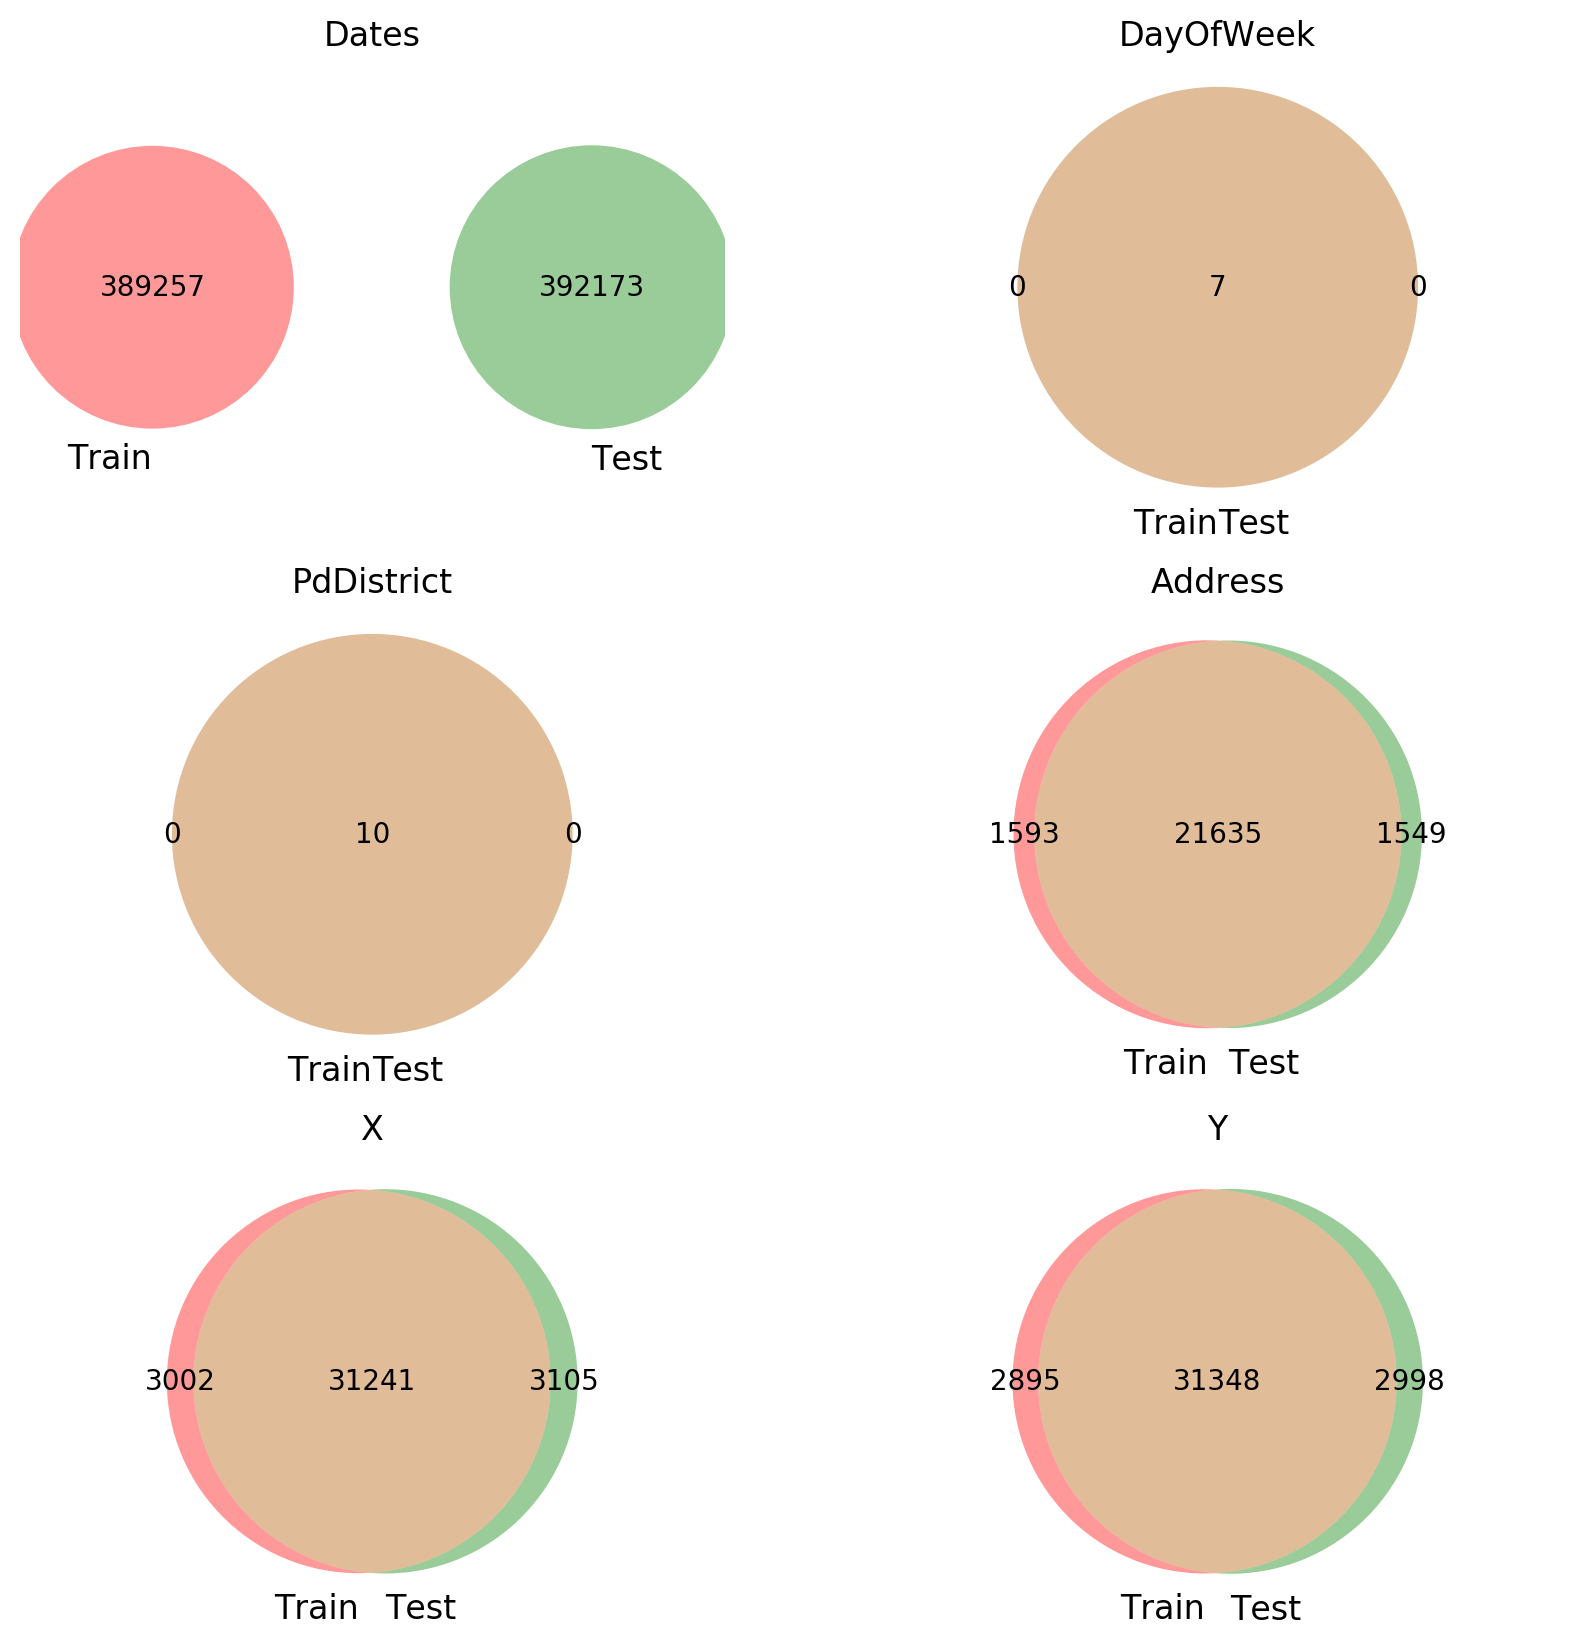
\includegraphics[width=0.5\textwidth]{overlap.png}
    \caption{属性重合度}
    \label{fig:overlap}
\end{figure}

注意到测试集和训练集的日期完全没有重合,
因此考虑将日期分割为“小时”,“日”,“月”,“年”四个属性,
经过统计,此时训练集和测试集完全重合。

\section{模型简介}

\subsection{逻辑回归}

由于需要预测的变量是分类的,本文首先尝试了最简单的逻辑回归模型。
Scikit Learn框架提供了Multinomial和One-versus-rest两种多分类回归模型,
提供了liblinear和newton-cg等多种求解算法和L1,L2两种正则项。
本文进行了多组对照实验对比其性能。

\begin{table*}[h]
    \centering
    \begin{tabular}{*{7}{r}}
        \hline
        模型& 算法& 正则项& 训练集loss& 测试集loss \\
        \hline
        OvR& liblinear& L2& 2.655& 2.656& \\
        OvR& liblinear& L1& & & \\
        OvR& newton-cg& L2& 2.641& 2.642& \\
        OvR& newton-cg& L1& & & \\
        Multinomial& newton-cg& L2& & & \\
        Multinomial& newton-cg& L1& & & \\
        \hline
    \end{tabular}
    \caption{逻辑回归分组实验}
    \label{tab:logsitic}
\end{table*}

\subsection{决策树}

决策树是一种机器学习模型,
它通过对训练数据进行分析,得到一个多次选择的分类器,
每一次根据样本的某个或某些属性进行决策,最终得到样本的分类。
决策树的每一个内部节点是样本的某一个特征,
从这个节点出发的每一个弧表示这个特征的可能取值,
如果指向另一个内部节点,则表示需要对另外一个样本特征进行决策,
如果指向叶子结点,则表示已经得到了对样本分类的结论。

与一个训练集不矛盾的决策树可能存在多个,也可能不存在,
因此需要定义评价函数来衡量决策树的性能。
常用的评价函数有信息增益(Information Gain)和基尼指数(Gini Impurity)等。
信息增益是指得知特征$X$的信息而是的类$Y$的信息的不确定性减少的程度。
特征$A$对训练集$D$的信息增益$g(D, A)$定义为集合$D$的经验熵$H(D)$
与特征$A$给定条件下$D$的经验条件熵$H(D|A)$之差,即

\begin{equation}
    g(D, A) = H(D) - H(D|A)
\end{equation}

训练集已知各个样本的分类,训练集的熵即这些分类的随机程度,
假设训练集样本共有$K$类,第$k$类的样本集合为$C_k$,则

\begin{equation}
    H(D) = -\sum_{k=1}^K\frac{|C_k|}{|D|}\mathrm{log}_2\frac{|C_k|}{|D|}
\end{equation}

如果根据特征$A$的取值来分类,可能会使得随机程度降低,
降低的程度反应了这个特征所包含的信息量。
假设$A$共有$n$种可能的取值,第$i$种取值的样本的子集为$D_i$,
再假设子集$D_i$中属于第$k$类的样本的集合为$D_{ik}$,则

\begin{equation}
    \begin{split}
        H(D|A) &= \sum_{i=1}^n\frac{|D_i|}{|D|}H(D_i) \\
               &= -\sum_{i=1}^n\frac{|D_i|}{|D|}\sum_{k=1}^K\frac{|D_{ik}|}{|D_i|}\mathrm{log}_2\frac{|D_{ik}|}{|D_i|}
    \end{split}
\end{equation}

已知信息增益,即可使用ID3和C4.5算法构建决策树\cite{statistics}。

为了避免决策树过于复杂导致过拟合,可以将决策树叶节点的个数加入损失作为正则项。

\begin{equation}
    \mathrm{loss} = \sum_{t=1}^{|T|}N_tH_t(T)+\alpha|T|
\end{equation}

其中$H_t(T)$表示第t个叶节点上的经验熵,$|T|$为叶节点的个数,$\alpha$为参数。

本文使用Scikit Learn库中的\lstinline[basicstyle=\ttfamily]|DecisionTreeClassifier|进行训练及预测\cite{scikit}。
实验发现,使用\lstinline[basicstyle=\ttfamily]|max_leaf_nodes|作为正则
可以显著提高测试集性能,但是再叠加AdaBoost则会降低训练集和测试集性能。
AdaBoost 详见后续章节。


\section{结果}

\begin{table}[h]
    \centering
    \begin{tabular}{ccc}
        \hline
        模型& 训练集loss& 测试集 loss \\
        \hline
        决策树& 0.238& 27.653 \\
        决策树(叶节点39个)& 2.538& 2.544 \\
        决策树(叶节点39个,Ada)& 3.372& 3.378 \\
        Gradient Boost& & 2.46332 \\
        \hline
    \end{tabular}
\end{table}

\bibliography{main}{}
\bibliographystyle{plain}

\end{document}

